% bei Standalone in documentclass noch:
% \RequirePackage{luatex85}

\documentclass[captions=tableheading, titlepage= firstiscover, parskip = half , bibliography=totoc]{scrartcl}
%paper = a5 für andere optinen
% titlepage= firstiscover
% bibliography=totoc für bibdateien
% parskip=half  Veränderung um Absätze zu verbessern

\usepackage{scrhack} % nach \documentclass
\usepackage[aux]{rerunfilecheck}
\usepackage{polyglossia}
\usepackage[style=numeric, backend=biber]{biblatex} % mit [style = alphabetic oder numeric] nach polyglossia
\addbibresource{lit.bib}
\setmainlanguage{german}

\usepackage[autostyle]{csquotes}
\usepackage{amsmath} % unverzichtbare Mathe-Befehle
\usepackage{amssymb} % viele Mathe-Symbole
\usepackage{mathtools} % Erweiterungen für amsmath
\usepackage{fontspec} % nach amssymb
% muss ins document: \usefonttheme{professionalfonts} % für Beamer Präsentationen
\usepackage{longtable}

\usepackage[
math-style=ISO,    % \
bold-style=ISO,    % |
sans-style=italic, % | ISO-Standard folgen
nabla=upright,     % |
partial=upright,   % /
]{unicode-math} % "Does exactly what it says on the tin."
\setmathfont{Latin Modern Math}
% \setmathfont{Tex Gyre Pagella Math} % alternativ

\usepackage[
% die folgenden 3 nur einschalten bei documenten
locale=DE,
separate-uncertainty=true, % Immer Fehler mit ±
per-mode=symbol-or-fraction, % m/s im Text, sonst \frac
]{siunitx}

% alternativ:
% per-mode=reciprocal, % m s^{-1}
% output-decimal-marker=., % . statt , für Dezimalzahlen

\usepackage[
version=4,
math-greek=default,
text-greek=default,
]{mhchem}

\usepackage[section, below]{placeins}
\usepackage{caption} % Captions schöner machen
\usepackage{graphicx}
\usepackage{grffile}
\usepackage{subcaption}

% \usepackage{showframe} Wenn man die Ramen sehen will

\usepackage{float}
\floatplacement{figure}{htbp}
\floatplacement{table}{htbp}

\usepackage{mhchem} %chemische Symbole Beispiel: \ce{^{227}_{90}Th+}


\usepackage{booktabs}

 \usepackage{microtype}
 \usepackage{xfrac}

 \usepackage{expl3}
 \usepackage{xparse}

 % \ExplSyntaxOn
 % \NewDocumentComman \I {}  %Befehl\I definieren, keine Argumente
 % {
 %    \symup{i}              %Ergebnis von \I
 % }
 % \ExplSyntaxOff

 \usepackage{pdflscape}
 \usepackage{mleftright}

 % Mit dem mathtools-Befehl \DeclarePairedDelimiter können Befehle erzeugen werden,
 % die Symbole um Ausdrücke setzen.
 % \DeclarePairedDelimiter{\abs}{\lvert}{\rvert}
 % \DeclarePairedDelimiter{\norm}{\lVert}{\rVert}
 % in Mathe:
 %\abs{x} \abs*{\frac{1}{x}}
 %\norm{\symbf{y}}

 % Für Physik IV und Quantenmechanik
 \DeclarePairedDelimiter{\bra}{\langle}{\rvert}
 \DeclarePairedDelimiter{\ket}{\lvert}{\rangle}
 % <name> <#arguments> <left> <right> <body>
 \DeclarePairedDelimiterX{\braket}[2]{\langle}{\rangle}{
 #1 \delimsize| #2
 }

\setlength{\delimitershortfall}{-1sp}

 \usepackage{tikz}
 \usepackage{tikz-feynman}

 \usepackage{csvsimple}
 % Tabellen mit \csvautobooktabular{"file"}
 % muss in table umgebung gesetzt werden


% \multicolumn{#Spalten}{Ausrichtung}{Inhalt}

\usepackage{hyperref}
\usepackage{bookmark}
\usepackage[shortcuts]{extdash} %nach hyperref, bookmark

\newcommand{\ua}[1]{_\symup{#1}}
\newcommand{\su}[1]{\symup{#1}}


\begin{document}

\section{Auswertung}

Bei den Messungen der Gegenstads- und der Bildgröße wurde ein Geodreieck verwendet.
Die weiteren Messwerte wurden an einem Lineal, welches an der Schiene integriert
ist, abgelesen. Es wird ein Ablesefehler von $\SI{0,05}{\centi\meter}$ angenommen.
Anhand der genommenen Messwerte wird die Linsengleichung \eqref{eqn:} und das
Abbildungsgesetz \eqref{eqn:} überprüft.
Die Messdaten sind in Tabelle \ref{tab:} dargestellt.

Damit das Abbildungsgesetz überprüft werden kann, sind die Mittelwerte der Messung
der Gegenstands- und der Bildweite verwendet worden. Als Fehler wurden die
Standardabweichungen des Mittelwertes angegeben.

\begin{description}
  \centering
  \item[$\frac{B}{G}=$]\SI{569(20)e-1}{\centi\meter}
  \item[$\frac{<b>}{<g>}=$]\SI{3929(14)e-2}{\centi\meter}
\end{description}

Die Mittelwerte $<b>$ und $<g>$ in die Linsengleichung \eqref{eqn:} eingesetzt,
ergeben die folgenden
Werte. Die Brennweite der Linse, ist vom Herstellen mit $\SI{10}{\centi\meter}$
angegeben.

\begin{description}
  \centering
  \item[$<f_1>\ua{gemessen}=$]\SI{10578(26)e-3}{\centi\meter}
\end{description}

Die Verbindungsgereaden, zu den Wertepaaren $(g_i|b_i)$, der Linse mit bekannter
Brennweite sind in \ref{fig:brennweite_bekannt}
dargestellt.

\begin{figure}
  \centering
  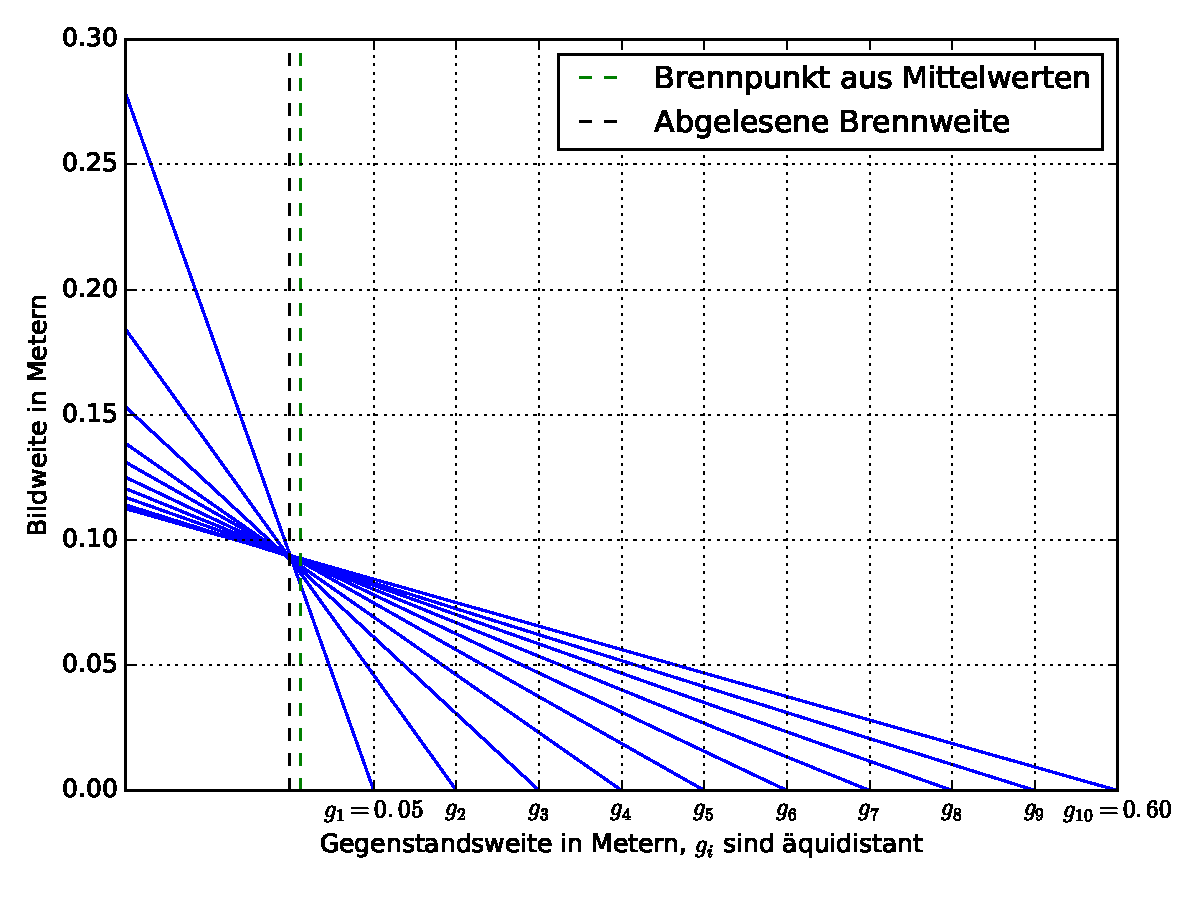
\includegraphics[width=\textwidth]{Messung1_brennnweite_bekannt.pdf}
  \caption{Wertepaare $(g_i|b_i)$ aufgetragen. Zudem ist der Mittelwert der gemessenen Brennweite, sowie der abgelesene Schnittpunkt der Geraden eingetragen.}
  \label{fig:brennweite_bekannt}
\end{figure}

Der Schnittpunkt der Geraden im Diagramm \ref{fig:brennweite_bekannt}
ist mit Hilfe des Mauscoursers abgelesen worden. Der Ablesefehler wird mit
$\SI{0,3}{\centi\meter}$ angegeben.
Der Schnittpunkt hat einen Wert von $S_1 = (\num{99(3)e-1}|\num{94(3)e-1})$.
Die Angaben sind in Centimetern.

Desweiteren wurde die Brennweite einer unbekannten Linse bestimmt.
Es wurde gleich verfahren, wie bei der Messung der bekannten Linse.

\begin{description}
  \centering
  \item[$<f_2>\ua{gemessen}=$]\SI{9028(3)e-2}{\centi\meter}
\end{description}

Das Diagramm \ref{fig:unbekannte_brennweite} zeigt die Verbindungsgeraden,
der Wertepaare der gemessenen $(g_i|b_i)$.

\begin{figure}
  \centering
  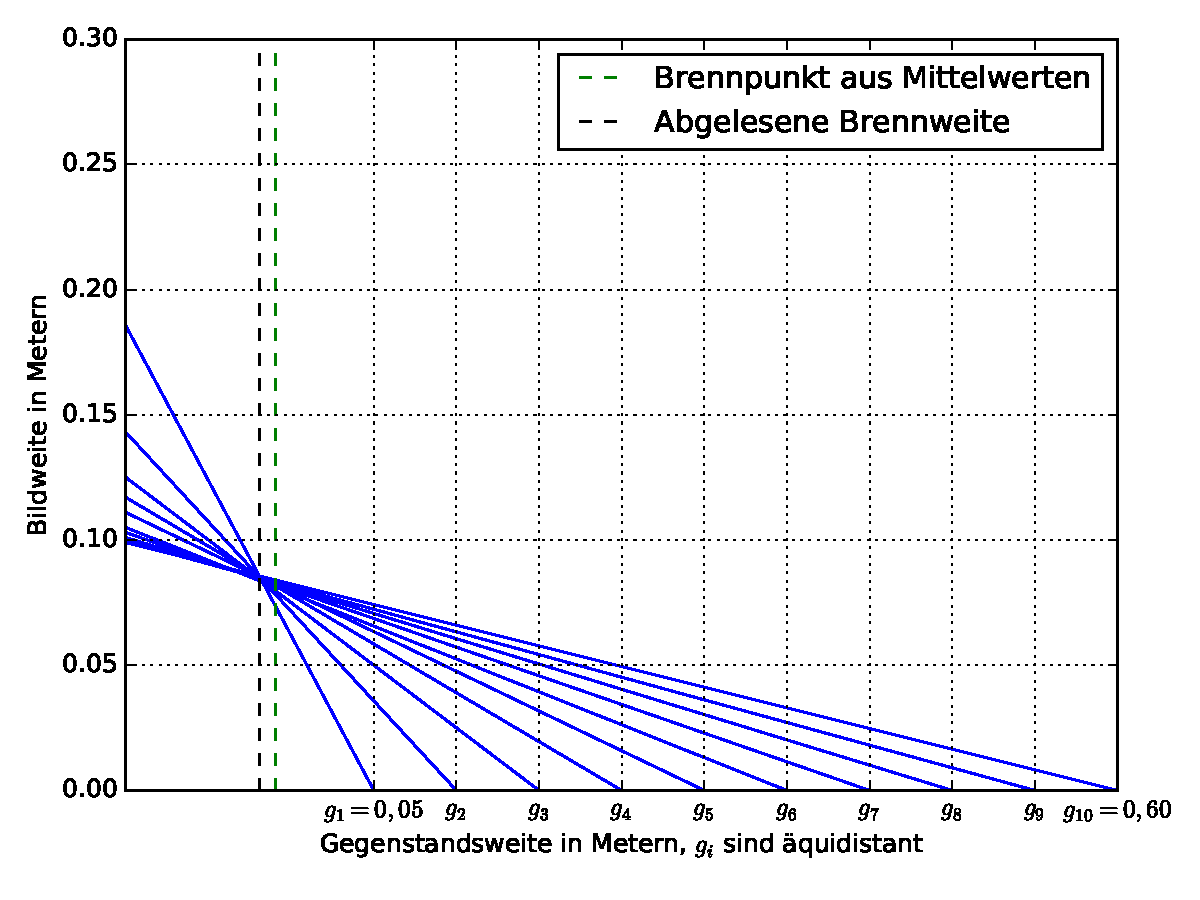
\includegraphics[width=\textwidth]{Messung2_unbekannte_brennweite.pdf}
  \caption{Wertepaare $(g_i|b_i)$ aufgetragen. Zudem ist der Mittelwert der gemessenen Brennweite, sowie der abgelesene Schnittpunkt der Geraden eingetragen.}
  \label{fig:unbekannte_brennweite}
\end{figure}

Der abgelesene Schnittpunkt ist gegeben mit $S_2 =
(\num{81(3)e-1}|\num{84(3)e-1})$. Die Angaben sind in Centimetern.

\subsection{Bestimmung der Brennweite nach Bessel}

Die Messdaten der Messung sind in Tabelle \ref{tab:bessel} dargestellt.
Damit der Datensatz größer ist, werden die Messdaten
von $b_1, g_1$ und $b_2, g_2$ verwendet. Theoretisch sind $b_1 = g_2$
und $b_2 = g_1$ identisch.

Die Mittelwerte der Messdaten wurden in die Formel \eqref{eqn:} eigetragen.
Daraus ergibt sich die folgende Brennweite.

\begin{equation}
  \centering
  \label{eqn:bessel_ergebnis}
  f\ua{Bessel}= \SI{9,67}{\centi\meter}
\end{equation}

Der Fehler von \eqref{eqn:bessel_ergebnis} ist, bezüglich der Messgenauigkeit,
vernachlässigbar klein und wird daher weggelassen.

Darüberhinaus wurde die chromatische Abberration untersucht.

\begin{align}
  \label{eqn:rot}
  f\ua{rot} &= \SI{967(1)e-2}{\centi\meter}\\
  \label{eqn:blau}
  f\ua{blau} &= \SI{966e-2}{\centi\meter}
\end{align}

Der Fehler bei \eqref{eqn:blau} ist, bezüglich der Messungenauigkeit,
zu vernachlässigen.

\subsection{Bestimmung der Brennweite von Linsensystemen nach Abbe}

Die Messdaten der Messung sind in Tabelle \ref{tab:} dargestellt.
Mit Formel \eqref{eqn:} ergeben sich daraus die folgenden Werte.

\begin{align}
  \label{eqn:brennweite_abbe_g}
  f\ua{g} &= \SI{1693(32)e-2}{\centi\meter} \\
  \label{eqn:hauptebene_h}
  f\ua{h} &= \SI{-938(95)e-2}{\centi\meter}\\
  \label{eqn:brennweite_abbe_b}
  f\ua{b} &= \SI{1442(17)e-2}{\centi\meter} \\
  \label{eqn:hauptebene_abbe_h_strich}
  f\ua{h´} &= \SI{1305(31)e-2}{\centi\meter}
\end{align}

\begin{figure}
  \centering
  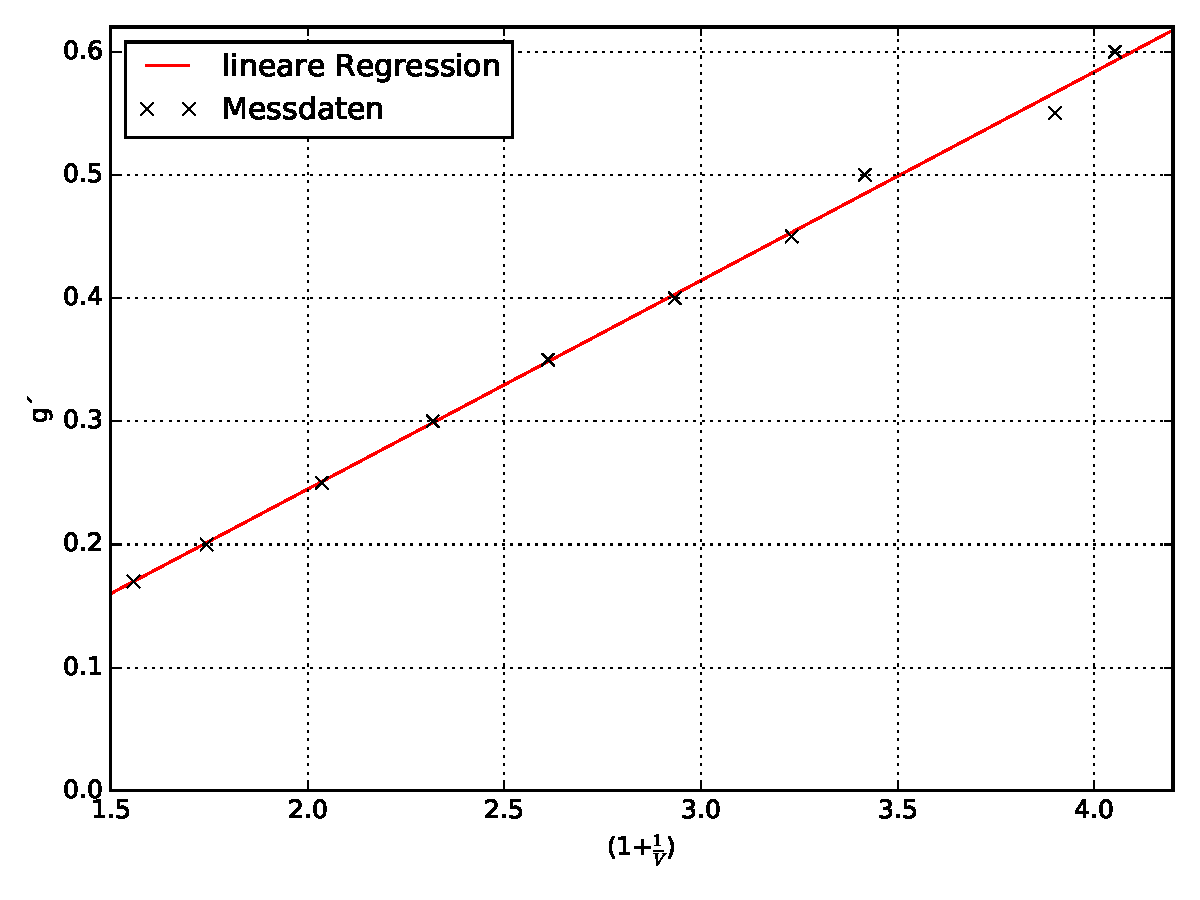
\includegraphics[width=\textwidth]{Messung_abbe_g.pdf}
  \caption{Wertepaare $(1 + \frac{1}{V_i}|g_i)$ mit linearer Regression.}
  \label{fig:abbe_g}
\end{figure}

\begin{figure}
  \centering
  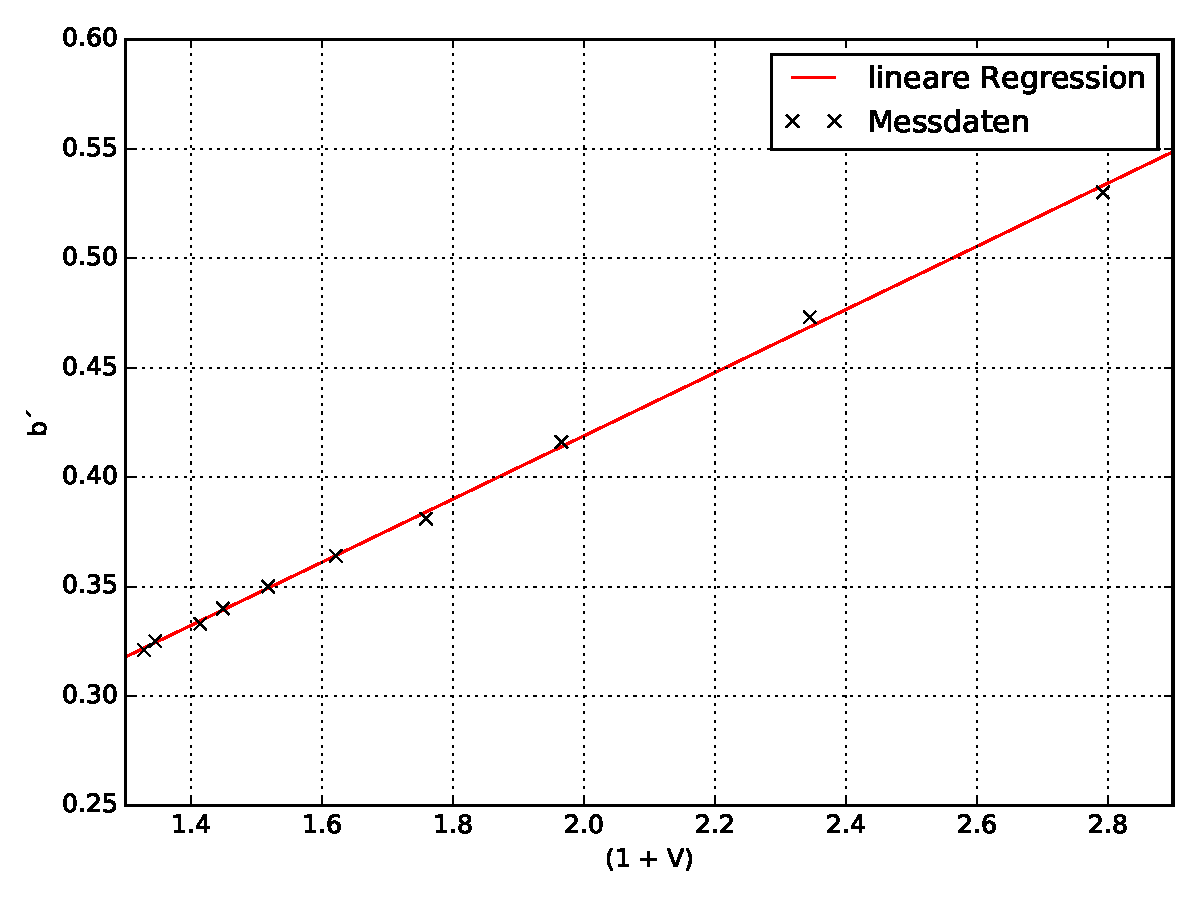
\includegraphics[width=\textwidth]{Messung_abbe_b.pdf}
  \caption{Wertepaare $(1 + V_i|b_i)$ mit linearer Regression.}
  \label{fig:abbe_b}
\end{figure}

\section{Diskussion}

Die Messgenauigkeit der Messung der Brennweite ist in Diagramm
\ref{fig:brennweite_bekannt} einzusehen. Bei einer hohen Messgenauigkeit haben
die eingetragenen Geraden einen gemeinsamen Schnittpunkt. Dies ist, unter
Berücksichtigung der Messunsicherheit, erreicht worden. Die Messung wird als
sehr präzise eingestuft. Die Messung weicht lediglich um
$\approx\SI{0,5}{\centi\meter}$ von der angegebenen Brennweite ab. Dies ebenfalls
auf eine hohe Präzision der Messung hin.

Als Linse mit unbekannter Brennweite wurde eine befüllbare Linse genommen. Die
Linse wurde über eine Spritze mit Wasser befüllt. Damit in der Linse ein konstanter
Druck gewährleistet wurde, musste die Spritze an einer definierten Person fixiert
werden. Die Fixierung wurde per hand bewerkstelligt. Die Messung war länger, womit
ein dauerhaft vollkommener konstanter Druck unwahrscheinlich scheint. Dadurch könnte
die Messung beeinflusst worden sein. Der in Diagramm
\ref{fig:unbekannte_brennweite} entstandene Schnittpunkt, weißt hingegen auf eine
hohe Messgenauigkeit hin.



Die chromatische Abberration ergab, dass die Brennweite bei blauer Lichtquelle
minimal kleiner ist, als bei roter Lichtquelle. Dies entspricht der Erwartung.

\end{document}
